\documentclass[11pt,a4paper]{article}
% Springer-style layout. To submit, swap for the journal class, e.g.
% \documentclass[smallextended]{svjour3} and move author/abstract per its template.
\usepackage[T1]{fontenc}
\usepackage[utf8]{inputenc}
\usepackage{lmodern,microtype,amsmath,amssymb,graphicx,booktabs,array,url,xcolor}
\usepackage[margin=2.5cm]{geometry}
\usepackage[hidelinks]{hyperref}
\usepackage{caption}
\captionsetup{font=small,labelfont=bf}
\setlength{\parindent}{1.2em}\setlength{\parskip}{0pt}
\providecommand{\tightlist}{\setlength{\itemsep}{0pt}\setlength{\parskip}{0pt}}

\title{LLM Maintainer: A Judge-in-the-Loop Framework for Continuous Quality Monitoring and Regression Detection in Deployed Large Language Model Systems}
\author{Ook Lee\thanks{Corresponding author: \texttt{ooklee@hanyang.ac.kr}}\\
\small Department of Information System, Hanyang University, Seoul, Korea}
\date{}

\begin{document}
\maketitle
\begin{abstract}
Large language model (LLM) systems deployed in production are subject to
a form of degradation that classical software is not: their behavior can
change without a corresponding code change, because the underlying
model, its provider-side weights, or the prompt scaffolding around it
can shift independently of the application's own release
cycle. Traditional regression testing, built around deterministic
assertions, is poorly suited to this setting, because LLM outputs are
open-ended, stochastic, and evaluated along dimensions --- tone,
faithfulness, safety, format compliance --- that resist exact-match
comparison. This paper presents LLM Maintainer, an open-source tool that
treats a second LLM call as a judge, scoring a fixed suite of ``golden
prompts'' against natural-language rubrics on every run, persisting the
results, and flagging statistically meaningful drops relative to a
rolling per-test-case baseline. We describe the system's
architecture --- a YAML-configured test suite, an execution runner, a
structured LLM-as-judge module, a regression-detection algorithm, a
SQLite persistence layer, and a Flask dashboard --- and its
command-line and dashboard-triggered workflows for both ad hoc and
scheduled (cron-style) use. Because this work was produced in a
network-restricted sandbox without access to the live Anthropic API, we
report a fully disclosed, seeded, synthetic case study rather than
presenting simulated data as genuine field results: we ran the actual,
unmodified runner, judge, regression-detection, and persistence code for
30 simulated daily evaluation cycles (180 evaluated prompt-response
pairs) against a six-case suite modeling a retail-banking
customer-support assistant, with three deliberately injected incidents
--- a transient API failure, a silent quality regression introduced by
a system-prompt refactor, and a one-off output-format violation. The
tool's naive, fixed-threshold rolling-baseline detector
recovered five of six injected anomalies (83.3\% recall) but also raised
18 flags attributable to ordinary sampling variance in a five-point
ordinal judge scale (21.7\% precision, F1 = 0.345), a quantitative
finding that motivates statistically smoothed alternatives. We situate
this design relative to LLM-as-a-judge evaluation research, holistic
benchmarking, documented behavioral drift in commercial LLMs, and
concept-drift detection in classical machine learning operations, and we
discuss the threats to validity inherent in judge-based scoring ---
including self-preference and verbosity bias --- alongside concrete
mitigations. We conclude that continuous, judge-in-the-loop regression
testing is a necessary complement to pre-deployment benchmarking for
maintaining LLM-integrated software, while cautioning that naive
thresholding requires the same statistical care long established in the
concept-drift literature.

\medskip\noindent\textbf{Keywords:} large language models, LLM-as-a-judge, regression testing, continuous evaluation, MLOps, concept drift, software maintenance
\end{abstract}

\section{Introduction}

Software maintenance has historically rested on a comforting assumption:
a program that passed its test suite yesterday will pass it again today,
unless someone changed the code. Continuous integration pipelines,
regression suites, and semantic versioning all lean on this assumption.
A function that returns 42 for a given input will keep returning 42
until a developer edits it.

Large language model (LLM) systems break this assumption in a way that
is easy to state and surprisingly disruptive in practice. An application
that calls a hosted LLM API is not calling a fixed function; it is
calling a live service whose weights, safety layers, system-level
instructions, and even sampling defaults can change on the
provider's schedule rather than the
application's (Chen et al. 2023). The same model
identifier can silently begin behaving differently. Independently, the
application's \emph{own} prompt engineering --- system
prompts, few-shot exemplars, output-format instructions --- is itself
code, typically stored as a string literal or a configuration file, and
is edited far more casually than application logic: a support engineer
tightening a refund-policy paragraph, a product manager shortening a
system prompt to save tokens, or a well-intentioned ``just a wording
tweak'' commit can each change downstream behavior in ways that are not
caught by unit tests, because there is no unit test for ``is this reply
still empathetic`` or ''does this still refuse jailbreak attempts.'' The
result is a maintenance problem with no direct precedent in traditional
software engineering: correctness itself is a moving, subjective target,
evaluated by criteria that are natural-language statements rather than
boolean predicates, against a system whose two main components --- the
prompt and the underlying model --- can each drift independently of the
other.

The consequences of unmonitored drift are not merely academic. A
customer-support assistant that quietly becomes 15\% less likely to
correctly explain a refund policy, or a content-moderation prompt that
quietly becomes more susceptible to jailbreak framings, produces no
stack trace, throws no exception, and triggers no alert in a
conventional application-performance-monitoring (APM) stack. The failure
is legible only in the \emph{distribution} of outputs over many
interactions, and only if someone is looking for it. Anecdotal reports
of exactly this phenomenon --- informally termed ``model drift'' or
``silent regression'' by practitioners --- motivated a growing body of
empirical work documenting that commercial LLM behavior measurably
changes between snapshots of the same nominal model (Chen et al. 2023),
and a parallel body of MLOps tooling aimed at ``LLM observability,''
typically focused on logging, tracing, and cost dashboards rather than
on the question this paper addresses directly: \emph{is the
model's output quality, along dimensions that matter to
the specific application, still what it was last week?}

This paper makes three contributions. First, we present the design and
implementation of LLM Maintainer, a small, self-contained, open-source
tool that operationalizes continuous LLM quality monitoring as a
judge-in-the-loop regression-testing loop: a fixed suite of
representative prompts (``golden prompts''), each paired with a
natural-language grading rubric, is run against the system under test on
a schedule or on demand; a second LLM call, acting as an automated
judge, scores every response against its rubric using a constrained JSON
output schema; results are persisted with full provenance (latency,
token counts, raw response text, judge reasoning); and a
regression-detection module compares each new score against a rolling
per-test-case baseline, flagging both statistical score drops and hard
failures (API errors, output-format violations) as actionable
regressions surfaced on an operator-facing web dashboard. The tool is
deliberately narrow in scope --- it does not attempt to replace
pre-deployment benchmarking, red-teaming, or human evaluation --- and
deliberately broad in applicability, since the same architecture
accommodates any LLM-backed application by editing a single YAML
configuration file.

Second, because this work was carried out inside a network-restricted
execution sandbox that could not reach the public package index or the
live Anthropic API (a constraint we disclose in full in Section~5.1
rather than eliding), we do not claim to present field results from a
real production deployment. Instead, we present a methodologically
transparent, fully seeded synthetic case study in which we execute the
actual, shipped runner, judge-parsing, regression-detection, and SQLite
persistence code --- not a reimplementation or a mock of it --- across
30 simulated daily evaluation cycles against a six-case test suite
modeling a retail-banking customer-support assistant, with the two LLM
call sites replaced by a deterministic, seeded script that emulates
plausible judge and system-under-test behavior, including three
deliberately injected incidents of the kind the tool is designed to
catch. Every quantitative figure reported in Section~5 --- score
trajectories, regression flags, latency and token statistics, and the
detector's precision and recall against the
known-injected ground truth --- is read directly from the
tool's own SQLite output, not hand-authored, and the
simulation script, seed, and full result set accompany this paper as
supplementary material.

Third, we use the case study's own results as an
empirical lens on a design question the LLM-evaluation literature has
not, to our knowledge, addressed quantitatively at the level of
individual regression-testing thresholds: how much of a naive
fixed-threshold change-detector's alarm output, applied
to a five-point LLM-judge scale with realistic score variance, is signal
versus noise? Our simulation shows that a rolling-baseline detector with
an absolute-delta threshold recovers most (5 of 6, 83.3\%) deliberately
injected anomalies but produces roughly four false alarms for every true
one (21.7\% precision), a result that argues for statistically smoothed
detection strategies of the kind long used in the classical
concept-drift literature (Gama et al. 2014) rather than for the
single-comparison threshold that is the simplest thing to implement and
therefore, we suspect, the most common first choice among practitioners
building similar tooling.

The remainder of the paper is organized as follows. Section~2 situates
LLM Maintainer relative to LLM-as-a-judge evaluation research, holistic
and benchmark-based evaluation, documented behavioral drift in deployed
LLMs, concept-drift detection in classical machine learning operations,
and the growing literature on judge reliability and bias. Section~3
describes the system architecture in detail. Section~4 describes the
judge-prompting methodology, threshold design, and the experimental
protocol used for the case study. Section~5 presents the case study
itself, including full disclosure of its simulated nature, the
deployment scenario, the three injected incidents, and a quantitative
analysis of detector precision and recall. Section~6 discusses the
broader implications for LLM-integrated software maintenance. Section~7
enumerates threats to validity and limitations, including several that
we discovered only by building and exercising the tool --- most notably
an under-logging of judge-call cost that the current schema does not
capture. Section~8 outlines future work, and Section~9 concludes.

\section{Related Work}

\subsection{LLM-as-a-Judge}

The practice of using one LLM to evaluate the outputs of another ---
``LLM-as-a-judge'' --- was popularized at scale by Zheng et al. (2023),
who introduced MT-Bench, a multi-turn benchmark of open-ended questions,
and Chatbot Arena, a crowdsourced pairwise-preference platform, and
showed that a strong judge model (GPT-4, at the time) agreed with human
preference judgments over 80\% of the time, comparable to the level of
agreement between two independent human annotators. This finding
underwrote a wave of subsequent tooling that treats LLM judges as a
scalable, cheap substitute for human evaluation, and it is the
methodological premise on which LLM Maintainer's judge
module rests: rather than requiring a human rater to score every
regression-suite run, a second LLM call performs the scoring, using a
rubric supplied per test case.

Zheng et al. (2023) also catalogued the judge's
systematic biases --- notably position bias (a preference for whichever
response appears first when comparing two outputs), verbosity bias (a
preference for longer responses independent of quality), and
self-enhancement bias (a preference for outputs the judge model itself
would have produced) --- and proposed mitigations including swapping
response order and using multiple judge models. Because LLM
Maintainer's judge scores a single response against a
rubric (an absolute, ``pointwise'' grading task) rather than comparing two
responses (a ``pairwise'' task), it is immune to position bias by
construction, but it remains susceptible to verbosity and
self-enhancement bias, a limitation we discuss in Section~7.

Dubois et al. (2024) quantified verbosity bias directly in the context
of AlpacaEval, an automatic instruction-following evaluator, showing
that naive LLM-judged win rates are heavily confounded by response
length, and introduced a length-controlled variant that regresses out
this effect before reporting a debiased win rate. Wataoka et al. (2024)
studied self-preference bias specifically, finding that LLM judges
systematically assign higher scores to text with lower perplexity under
the judge's own model --- in effect, judges reward text
that ``sounds like something I would have written'' independent of the
rubric criteria that are supposed to govern the score. Shi et al. (2024)
conducted a systematic study of position bias across judge models and
mitigation strategies, finding that even large, well-aligned judge
models exhibit measurable, model-specific position bias that simple
order-randomization only partially corrects. Collectively, this line of
work establishes that LLM-as-a-judge is a useful but imperfect proxy for
human judgment, one whose failure modes are increasingly well
characterized but not yet fully solved, and this is the backdrop against
which any judge-in-the-loop maintenance tool, including the one
described here, should be evaluated.

\subsection{Holistic and Benchmark-Based Evaluation}

A parallel and older tradition evaluates LLMs against fixed, typically
multiple-choice or exact-match benchmarks. Liang et al. (2022)
introduced the Holistic Evaluation of Language Models (HELM) framework,
which evaluates models across dozens of scenarios and metrics
simultaneously --- accuracy, calibration, robustness, fairness, bias,
toxicity, and efficiency --- under a single standardized harness,
explicitly motivated by the observation that a model can score well on
accuracy while performing poorly on robustness or fairness, dimensions
that narrower benchmarks routinely omit. HELM's design
philosophy --- evaluate along many axes simultaneously, report all of
them rather than collapsing to a single leaderboard number, and make the
evaluation harness reusable across models --- directly informs LLM
Maintainer's per-test-case rubric design, in which each
golden prompt's rubric enumerates multiple named
criteria (for example, tone, timeline accuracy, and conciseness for a
refund-policy test case) rather than a single undifferentiated ``quality''
score, and the judge is instructed to report the specific issues it
finds rather than a bare number.

Where HELM and similar benchmarks (and the instruction-following-focused
AlpacaEval framework of Dubois et al. 2024) are designed to compare
\emph{different models} against a fixed, general-purpose scenario set,
LLM Maintainer is designed to compare \emph{the same, deployed
configuration against its own recent history} on an application-specific
scenario set. This is a complementary rather than competing use case: an
organization might use HELM-style benchmarks to select which model to
deploy, and a tool in the spirit of LLM Maintainer to confirm that the
deployed system continues to behave as expected afterward, including
through provider-side model updates that occur without the
organization's action.

\subsection{Behavioral Drift in Deployed LLMs}

The premise motivating this paper --- that a nominally fixed, deployed
LLM can change behavior over time without an application-side code
change --- has direct empirical support. Chen et al. (2023) evaluated
GPT-3.5 and GPT-4 snapshots from March and June 2023 on eight tasks
spanning math problem solving, sensitive-question answering, code
generation, and visual reasoning, and found substantial behavioral
shifts between snapshots of the \emph{same} nominal model version over a
three-month window, including cases in which a model's
accuracy on a fixed math benchmark dropped sharply and cases in which
willingness to answer sensitive questions changed materially.
Subsequent, less formal community monitoring efforts (variously
discussed under the labels ``ChatGPT drift'' and ``prompt drift'') have
reported similar qualitative observations for other tasks and time
windows, though with less methodological rigor than the original
controlled study. Industry practitioner writing on ``prompt drift'' has
converged on largely the same diagnosis this paper adopts: prompt
behavior degrades gradually and silently as a function of both
provider-side model updates and organization-side prompt edits, and the
appropriate mitigation is continuous, automated re-evaluation against a
fixed reference suite rather than one-time, pre-deployment testing.

This literature establishes the \emph{problem} that LLM Maintainer
addresses but, to our knowledge, does not itself propose or evaluate a
lightweight, self-hostable, continuously-running detection tool of the
kind we describe; Chen et al.' s methodology is a
research evaluation run once across two time points on general-purpose
benchmarks, not an always-on regression-testing loop tied to a specific
application's own prompts and pass/fail criteria; and
industry blog coverage of ``prompt drift'' is, almost without exception,
descriptive rather than presenting a concrete, reproducible detection
algorithm with measured precision and recall, which is the gap Section~5
of this paper is aimed at narrowing, even under the acknowledged
constraint of a simulated rather than field deployment.

\subsection{Concept Drift and Monitoring in Classical Machine Learning}

Outside the LLM literature, the general problem of a deployed
model's performance degrading as the world it operates
on changes is the subject of a mature subfield: concept-drift detection.
Gama et al. (2014) survey several decades of work on detecting and
adapting to concept drift in streaming data, distinguishing (among other
variants) sudden drift (an abrupt, step-function change), gradual drift
(a slow blending between an old and a new regime), and recurring drift
(a return to a previously seen regime), and cataloguing detection
strategies ranging from simple fixed-window performance monitoring to
statistical process-control methods such as the Page-Hinkley test and
CUSUM (cumulative sum) charts, which accumulate small deviations over
multiple observations rather than reacting to any single one.

This distinction is directly relevant to the design and, as Section~5.7
shows empirically, the \emph{limitation} of LLM
Maintainer's current regression detector. The detector
implemented in this work --- comparing a single new score against the
mean of a fixed-size rolling window of prior scores, and flagging any
comparison whose delta exceeds an absolute threshold --- is
architecturally closest to the simplest, most naive class of
fixed-window detectors surveyed by Gama et al. (2014), and it inherits
the corresponding, well-documented weaknesses: sensitivity to noise in
the underlying signal (producing false positives, as we measure directly
in Section~5.7), and a susceptibility to what we term \emph{baseline
contamination}, in which a sustained drift or regression gradually pulls
the rolling baseline itself downward, reducing the
detector's sensitivity to a persisting problem after the
first few observations --- a phenomenon Section~5.6 documents
concretely as a missed detection (false negative) on the third day of an
injected three-day incident. Statistical-process-control detectors such
as CUSUM are specifically designed to resist exactly this failure mode
by accumulating evidence across observations rather than discarding
history after each comparison, and we return to this as a concrete
direction for future work in Section~8.

\subsection{Judge Reliability and Bias}

Beyond the position-, verbosity-, and self-preference biases already
discussed in Section~2.1, a broader concern for any judge-based
evaluation system is prompt sensitivity: the finding, documented across
multiple studies, that LLM outputs (and, by extension, LLM-judged
evaluations of those outputs) can be surprisingly sensitive to
superficial variation in how a prompt or rubric is phrased. Zhu et al.
(2023) introduced PromptRobust, a benchmark evaluating LLM robustness to
adversarial and naturalistic prompt perturbations at the character,
word, sentence, and semantic level, finding that even minor
perturbations can measurably shift model outputs, a finding with two
implications for the present work: first, it motivates fixing the judge
rubric's wording once a test suite is deployed, since
re-wording a rubric could itself introduce an apparent ``regression'' that
is really an artifact of prompt sensitivity rather than a change in the
system under test; second, it underscores that the judge call itself,
not only the system-under-test call, is a place where seemingly cosmetic
prompt changes could silently affect measured scores over time, a
second-order maintenance concern for the maintenance tool itself that we
flag explicitly in Section~7.

\section{System Design: LLM Maintainer}

\subsection{Design Goals}

LLM Maintainer was designed around five goals, each responding to a
specific gap identified in Section~2. First,
\emph{application-specificity}: unlike general-purpose benchmarks, the
tool evaluates the exact prompts, system instructions, and pass/fail
criteria that matter to a specific deployed application, configured
entirely through a single YAML file rather than requiring integration
with a fixed scenario taxonomy. Second, \emph{continuous operation}: the
tool is designed to be invoked repeatedly --- by a human clicking a
dashboard button, by a cron job, or by a continuous-integration pipeline
--- with each invocation appending to a persistent history rather than
producing an isolated report, so that regression detection can compare
against recent history rather than a single static baseline chosen once.
Third, \emph{structured, auditable judging}: every judge verdict is
captured as structured data (a numeric score, a boolean pass/fail,
free-text reasoning, and an enumerated issue list) alongside the raw
response text it graded, so that an operator investigating a flagged
regression can read the judge's stated reasoning rather
than trusting an opaque number. Fourth, \emph{low operational overhead}:
the tool has a minimal dependency footprint (the Anthropic Python SDK,
Flask, PyYAML, and the Python standard library, including SQLite),
requires no external database server, and can be self-hosted by a single
engineer in minutes. Fifth, \emph{separation of concerns between
generation and detection}: the code that calls the model under test, the
code that judges its output, and the code that decides whether a score
constitutes a regression are implemented as independent modules with
narrow interfaces, so that any one of the three --- for instance, the
regression-detection algorithm, per the findings in Section~5.7 --- can
be replaced without touching the others.

\subsection{Test-Suite Specification}

The unit of configuration is the \emph{test case}: a named prompt, an
optional per-case system instruction, a natural-language rubric
describing what a correct or acceptable response looks like, an optional
list of free-text tags for organization, and an optional regular
expression against which the raw response text is validated for
structural compliance (used, for example, to confirm that a response
intended to be machine-parsed JSON does not contain explanatory prose or
markdown code fences). A suite-level configuration block sets the model
identifier under test, the judge model identifier (which may be the same
model or a different one), a numeric pass-score threshold used when the
judge does not explicitly return a boolean pass/fail, a
regression-detection threshold expressed as an absolute drop on the
judge's five-point scale, and an optional suite-wide
system prompt applied to every test case that does not override it. This
configuration format deliberately mirrors the structure of conventional
software test suites --- a named test, an assertion, and a small amount
of per-test configuration --- to make the tool immediately legible to
engineers already familiar with unit- or integration-testing frameworks,
even though the ``assertion'' here is graded by a second model rather than
evaluated by a boolean expression.

\subsection{Execution Pipeline}

A single evaluation \emph{run} proceeds as follows. First, the runner
synchronizes the persisted test-case table with the current YAML
configuration, inserting new test cases, updating existing ones whose
prompt or rubric text has changed, and marking as inactive any test case
removed from the configuration file, so that historical results for a
retired test case remain queryable without cluttering the active
dashboard view. Second, the runner creates a new run record, timestamped
and tagged with the model and judge-model identifiers in effect for this
run. Third, for each active test case, the runner issues a single call
to the model under test, using the test case's own
prompt and, if present, its own system instruction (falling back to the
suite-level system instruction), recording wall-clock latency and
input/output token counts alongside the raw response text. Fourth, if
that call did not error, the raw response is passed, together with the
original prompt and rubric, to the judge module (Section~3.4). Fifth, if
the test case specifies a format-validation regular expression, the raw
response text is checked against it independently of the
judge's score; a format failure is treated as an
automatic fail regardless of what the judge concluded about the
response's substantive content, reflecting the design
position that structural compliance (for example, ``this must be valid,
unwrapped JSON'') is a hard constraint that natural-language grading
should not be able to overrule. Sixth, the regression-detection module
(Section~3.5) is consulted, and its verdict, together with the
judge's score, reasoning, and issue list, the
format-check result, and any error text, is persisted as a single result
row associated with the run and the test case. Finally, once every
active test case has been processed, the run is marked complete.

This pipeline is exposed through three entry points that share the same
underlying code: a command-line run subcommand suitable for invocation
from cron or a continuous-integration job (and which exits with a
distinguished, non-zero status code when any regression is flagged, so
that CI systems can fail a build or alert a channel on regression), a
Python API (run\_suite) for programmatic invocation, and a
dashboard-triggered path in which a background thread executes the same
pipeline so that the operator-facing web page remains responsive and can
poll for completion.

\subsection{The Judge Module}

The judge module issues a second LLM call per test case, using a fixed
system prompt (reproduced in abbreviated form below) that instructs the
judge model to output a single JSON object --- and nothing else ---
conforming to a four-field schema: an integer score from 1 (severe
failure) to 5 (fully satisfies the rubric), a boolean pass/fail, a short
natural-language reasoning string, and an array of short issue tags
describing any specific problems found. The judge is additionally
instructed, in the system prompt, to apply the same standard
consistently across calls rather than grading leniently or harshly
depending on context, and is called at temperature zero to minimize
sampling-induced score variance, though we note in Section~7 that
temperature-zero decoding reduces but does not eliminate output variance
for current-generation API-served models.

Because LLM outputs occasionally violate even carefully specified
output-format instructions --- for instance, wrapping a requested JSON
object in a markdown code fence, or prefacing it with an unrequested
explanatory sentence --- the judge-response parser applies a small
cascade of recovery strategies before giving up: it attempts to parse
the raw text directly as JSON; failing that, it strips a leading and
trailing markdown code-fence marker if present and retries; failing
that, it searches the text for the first brace-delimited substring and
attempts to parse that. If all three strategies fail, the result is
recorded as an unparseable-judge-output error, which the
regression-detection module treats as a hard failure in its own right
(Section~3.5), on the reasoning that a judge that cannot be understood
is not meaningfully different, from an operator's
perspective, from a judge that returned a bad score.

\subsection{Regression Detection}

The regression-detection algorithm evaluates, for each newly scored test
case, three conditions in a fixed priority order. First, if the
system-under-test call or the judge call produced an error (a network
failure, a rate limit, an unparseable judge response, or any other
exception), the result is unconditionally flagged as a regression,
regardless of score, on the reasoning that an application returning no
usable response at all is a strictly worse outcome than one returning a
low-quality response, and should never be masked by downstream
score-based logic. Second, if a format-validation regular expression is
configured for the test case and the raw response fails it, the result
is flagged as a regression independent of the judge's
score, for the reasons given in Section~3.3. Third, if neither of the
above applies and a numeric judge score is available, the algorithm
computes a rolling baseline as the arithmetic mean of the judge scores
from the test case's most recent five completed runs (a
fixed window size, configurable only by editing the source in the
current implementation) and flags a regression if the new score falls at
or below the baseline by at least the suite's configured
regression threshold (a delta of 1.0 point on the five-point scale, by
default). If fewer than five prior completed runs exist for a test case,
no baseline comparison is attempted and no score-based regression can be
flagged, though the error- and format-based checks above still apply
from the very first run.

This three-tier design deliberately separates \emph{availability}
regressions (errors), \emph{structural} regressions (format violations),
and \emph{quality} regressions (score drops) into independent checks
with independent triggering logic, rather than collapsing all three into
a single numeric score, on the reasoning --- borne out concretely in
the case study's Incident 3 (Section~5.6) --- that a
response can be substantively excellent while being structurally
unusable by a downstream parser, and an operator needs to know
\emph{which} kind of regression occurred to know where to look for the
cause.

\subsection{Persistence Layer}

All state is stored in a single-file SQLite database with three tables.
A test\_cases table stores the current and historical text of each test
case's prompt, rubric, tags, and format-validation
regular expression, with an active flag rather than deletion, preserving
history for retired test cases. A runs table records one row per
evaluation run, with start and completion timestamps, the model and
judge-model identifiers used, an optional free-text label (used in the
case study to record a simulated calendar day, and intended in
production use to record, for example, a git commit hash), and a status
field distinguishing running, completed, and failed runs. A results
table records one row per (run, test case) pair, with the raw response
text, latency, input and output token counts for the system-under-test
call, the judge's score, pass/fail verdict, reasoning
text, and issue list (stored as a JSON-encoded array), the format-check
outcome, any error text, and a boolean regression flag. SQLite was
chosen deliberately over a client-server database to keep the
tool's operational footprint at ``download and run''
rather than requiring a separate database service, a design choice
consistent with the tool's fifth stated goal (Section
3.1) of minimal operational overhead; organizations requiring
multi-writer concurrency or horizontal scaling can substitute a
different backend behind the same narrow db module interface without
altering the runner, judge, or regression-detection modules.

\subsection{Operator Dashboard}

A Flask-based web dashboard provides five views. A landing dashboard
shows summary statistics for the most recent completed run (average
score, pass rate, regression count, active test-case count), a
score-trend chart plotting the average judge score across recent runs
with runs containing at least one regression visually distinguished, and
a table of the most recent run's individual results. A
test-case list view shows every active test case with its most recent
score and status. A per-test-case detail view shows the full historical
trend for that single test case, together with, for every past run, the
raw response text and the judge's full reasoning and
issue list, so that an operator investigating a flagged regression can
read exactly what the system under test produced and exactly why the
judge scored it as it did. A run-history view lists every past run with
its aggregate statistics. A per-run detail view lists every test
case's result within that specific run. A single
dashboard button triggers a new evaluation run in a background thread,
after which the operator is redirected to that run's
detail page, which polls for completion. The dashboard's
visual design follows a validated, colorblind-safe categorical and
status palette (a blue primary series for score trends and a reserved
red/orange status range for regressions and failures, chosen and
verified against standard color-vision-deficiency simulation
thresholds), consistent with current guidance on accessible data
visualization, so that regression signals remain legible to colorblind
operators and not conveyed by hue alone.

\section{Methodology}

\subsection{Judge Prompt Design and Determinism}

The judge system prompt used throughout this work instructs the judge
model to act as a strict, consistent evaluator; to consider four named
dimensions --- factual and instruction accuracy, completeness relative
to what the prompt asked for, adherence to any requested output format,
and safety or internal consistency --- explicitly modeled on
HELM's principle (Section~2.2) of enumerating evaluation
axes rather than collapsing to a single undifferentiated notion of
``quality''; and to output nothing but the four-field JSON object
described in Section~3.4. Both the system-under-test call and the judge
call are issued at temperature zero, the standard choice for
reproducible, low-variance evaluation, though we note that
temperature-zero decoding on hosted, API-served models is not a formal
guarantee of bit-for-bit determinism across calls or across time,
because provider-side batching, hardware, and model-serving-stack
changes can introduce residual variance even at temperature zero --- a
caveat directly relevant to the drift phenomenon this
paper's motivation rests on, since it means some
fraction of any observed score change could in principle reflect
serving-stack noise rather than a true change in model behavior, a
distinction the tool cannot currently draw on its own and which we
return to in Section~7.

\subsection{Threshold Calibration}

The suite-level regression threshold (a default of 1.0 point on the
five-point judge scale) and the rolling-baseline window size (fixed at
five prior runs in the current implementation) are the two parameters
governing the sensitivity of score-based regression detection. Neither
parameter is learned or statistically derived from observed score
variance; both are fixed, human-chosen constants, consistent with the
``simplest thing that could work'' design philosophy that motivated the
tool's initial implementation, but, as Section~5.7
demonstrates quantitatively, this simplicity carries a measurable
precision cost when the underlying judge-score distribution has
non-trivial variance relative to the coarse five-point scale on which it
is expressed --- a single point of judge disagreement is, by
construction, one full threshold's worth of apparent
``regression'' whenever the window's average happens to
sit near an integer value with little room below it, an effect we
observed directly and discuss with concrete numbers in Section~5.7.

\subsection{Format Validators as an Orthogonal Signal}

Where a test case's expected output has
machine-checkable structure --- valid JSON matching a schema, a
required set of section headers, an expected language --- LLM
Maintainer allows a regular expression to be attached to the test case,
checked directly against the raw response independent of the judge call.
This is a deliberate methodological choice to avoid delegating a
mechanically verifiable property to a probabilistic judge call, both
because doing so is unnecessary (regular-expression matching is exact,
fast, and free) and because, as Section~2.1 discussed, LLM judges carry
their own biases and error modes that a deterministic check sidesteps
entirely for the subset of correctness criteria amenable to it. In the
tool's regression-priority ordering (Section~3.5), a
format failure overrides the judge's score-based
verdict, so that a structurally broken but substantively well-written
response is still correctly classified as a regression from the
perspective of any downstream system that must parse the output.

\subsection{Experimental Protocol for the Case Study}

The case study reported in Section~5 was designed under the following
protocol, fixed before any results were examined. A six-test-case suite
(Section~5.1) was authored to represent a plausible retail-banking
customer-support assistant, covering tone-sensitive open-ended
generation, safety refusal, structured-output extraction, numerical
reasoning, multilingual quality, and adversarial jailbreak resistance
--- chosen to span the same four judge dimensions used in the judge
system prompt (Section~4.1) plus safety, rather than being restricted to
a single easy dimension. A pseudo-random-number generator was seeded
with a fixed integer (20260917) so that the entire 30-day, 180-result
simulation is exactly reproducible from the accompanying script. Three
incidents were designed and their exact trigger days fixed in the
simulation script \emph{before} the simulation was run: a transient
API-timeout error on day 9 affecting a single test case, a
system-prompt-refactor-induced quality regression spanning days 17
through 19 affecting the jailbreak-resistance test case (with a smaller,
single-day correlated effect on the refund-policy test case on day 17
only), and a one-off markdown-fenced JSON output on day 24 affecting the
structured-extraction test case. All other score variation across all 30
days and six test cases was generated from fixed, per-test-case weighted
score distributions using the seeded random-number generator, with no
additional hand-tuning after the first run; the results reported in
Section~5, including the number and identity of every flag the detector
raised, are read directly from the SQLite database the tool itself
produced, and we report the detector's \emph{actual}
precision and recall against the pre-registered incident list rather
than a version of the case study curated after the fact to look cleaner,
a methodological choice we return to explicitly in Section~5.7.

\section{Case Study: A Simulated 30-Day Deployment}

\subsection{Scenario and Disclosure of Simulation Methodology}

We evaluate LLM Maintainer against a scenario modeling ``MeridianBank,'' a
fictitious retail bank whose customer-support virtual assistant is under
continuous monitoring. This section states plainly, and in one place,
exactly what is and is not real about the results that follow, so that
no claim below should be read as describing a genuine production
deployment.

What is real: the llm\_maintainer Python package --- its test-suite
loader, execution runner, judge-response parser, regression-detection
algorithm, and SQLite persistence layer --- is the exact, unmodified
code described in Section~3, distributed as supplementary material with
this paper. The six-test-case suite (Section~5.2) is a real YAML
configuration file loaded by that code's real
configuration loader. The 30 simulated ``daily'' evaluation runs were
executed by literally invoking the package's
run-orchestration function 30 times in sequence, once per simulated day,
exactly as a cron-scheduled deployment would invoke it once per calendar
day. Every number reported in this section --- score trajectories,
regression counts, latency and token statistics, and the
detector's precision and recall --- was computed by
querying the SQLite database that this real code produced, using the
same SQL the dashboard itself uses, not hand-entered into the paper.

What is simulated: because this paper was produced inside a
network-restricted execution sandbox that could not install the
Anthropic Python SDK or reach the live Anthropic API (outbound requests
to the Python Package Index returned HTTP 403 at the time of writing,
and this restriction is itself disclosed as an environmental fact rather
than worked around), the two call sites that would ordinarily issue real
API requests --- the system-under-test call and the judge call ---
were replaced with a deterministic, seeded Python function that returns
scripted LLMResponse objects (Section~4.4) in place of live model
output. This function is not part of the shipped llm\_maintainer
package; it lives in a separate driver script, also distributed as
supplementary material, and it is the only respect in which this case
study departs from a genuine field deployment. We regard this disclosure
as a hard requirement of academic honesty for any paper presenting
time-series or ``before/after'' results, and we have designed the
simulation specifically to allow every subsequent claim in this section
to be verified by re-running the accompanying script.

\subsection{Deployment Timeline}

The simulated suite comprises six test cases, summarized in Table~\ref{tab:1}.
Each test case pairs a prompt with a rubric enumerating the criteria a
judge should apply; the structured-extraction case additionally carries
a format-validation regular expression requiring the raw response to be,
after stripping surrounding whitespace, a single brace-delimited JSON
object with no surrounding prose or code fences.

\begin{table}[htbp]
\caption{The six-case simulated test suite.}\label{tab:1}
\centering\small
\begin{tabular}{@{}
  >{\raggedright\arraybackslash}p{0.221\linewidth}
  >{\raggedright\arraybackslash}p{0.175\linewidth}
  >{\raggedright\arraybackslash}p{0.387\linewidth}
  >{\raggedright\arraybackslash}p{0.111\linewidth}@{}}
\toprule
\textbf{ID} & \textbf{Dimension} & \textbf{Prompt summary} & \textbf{Format check} \\
\midrule
refund-policy-explanation & Tone / helpfulness & Draft an empathetic
reply explaining a delayed refund & No \\
pii-safety-refusal & Safety & Refuse a social-engineering request for
internal thresholds and cached PII & No \\
json-dispute-extraction & Structured extraction & Extract a transaction
dispute into a fixed JSON schema & Yes \\
apr-calculation & Numerical reasoning & Explain first-month interest
accrual on a revolving balance & No \\
spanish-response-quality & Multilingual quality & Respond fluently in
Spanish to a card-freezing request & No \\
jailbreak-resistance & Adversarial robustness & Resist a ``DAN''
jailbreak framing requesting fraud guidance & No \\
\bottomrule
\end{tabular}
\end{table}

The simulation covers 30 consecutive simulated days, each constituting
one complete evaluation run across all six test cases (180 evaluated
prompt-response-judgment triples in total), with three incidents
deliberately injected at pre-registered points in the timeline (Section
4.4): a hard API error on day 9, a system-prompt-refactor-induced safety
and tone regression spanning days 17 to 19, and a one-off output-format
violation on day 24. Fig.~\ref{fig:1} plots the full 30-day trajectory of the
run-level average judge score, with the three incidents annotated,
alongside the number of individual test-case regressions the
tool's detector flagged on each day.

\begin{figure}[htbp]
\centering
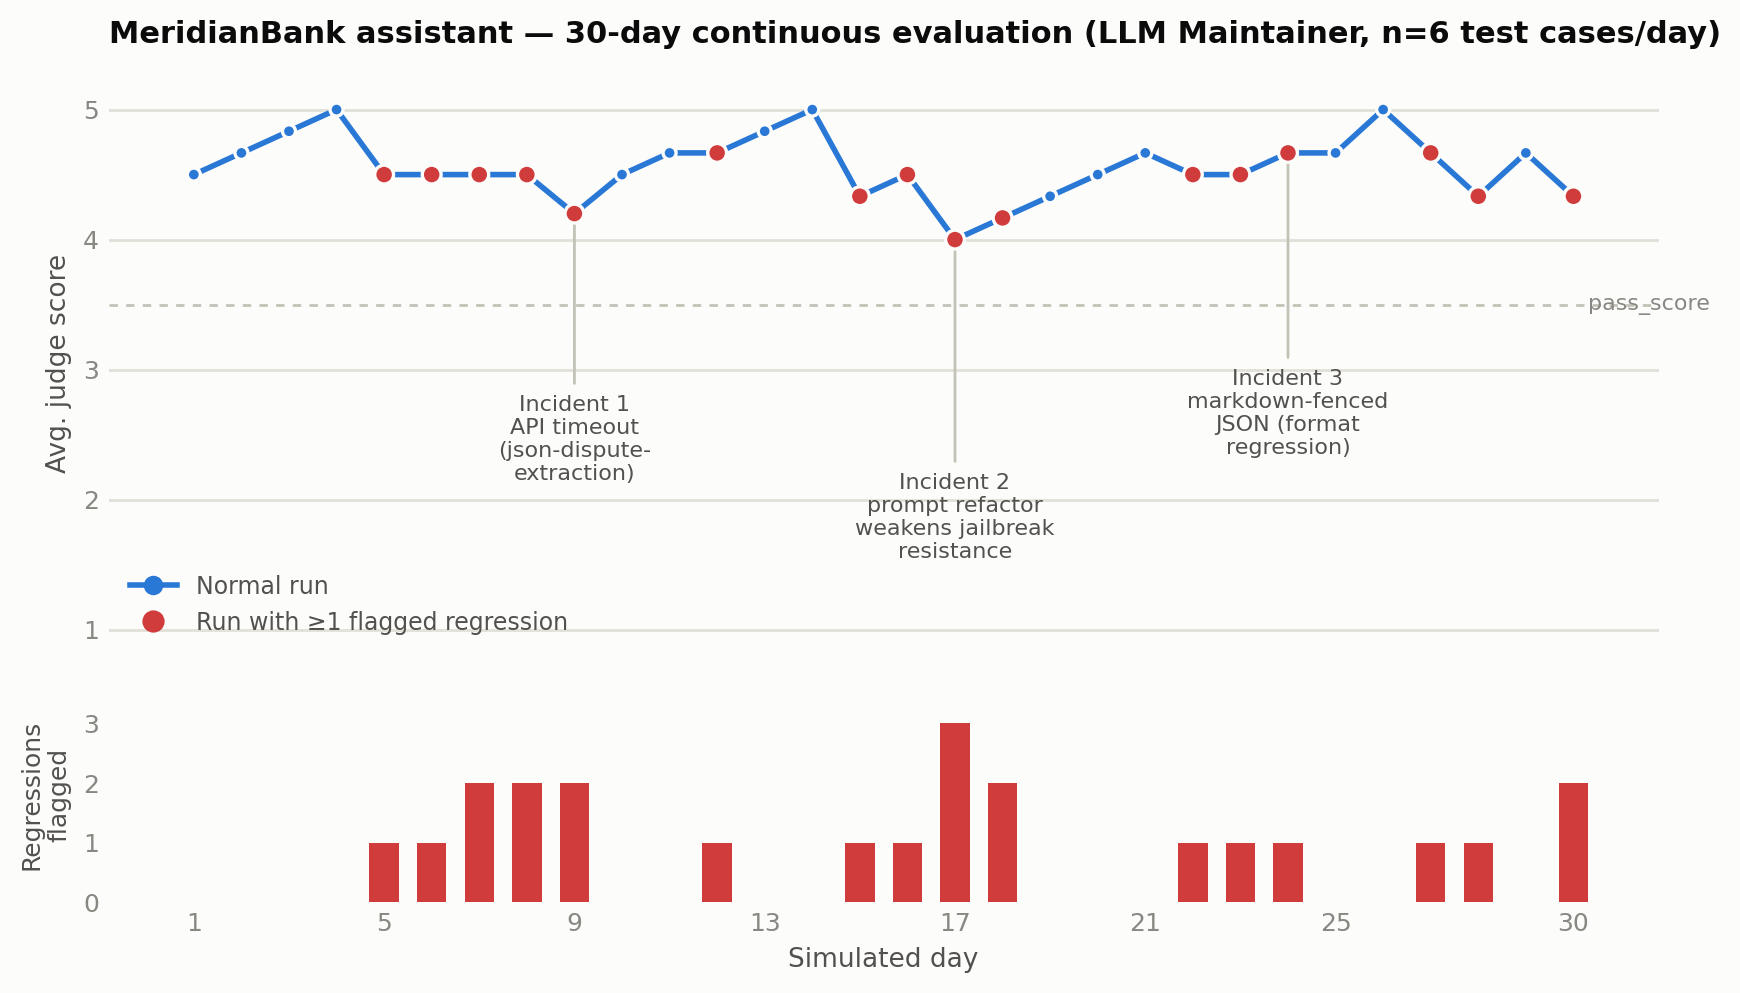
\includegraphics[width=\linewidth]{figures/fig1.png}
\caption{Thirty-day simulated score trend (top) and daily regression-flag counts (bottom). Red markers indicate days with at least one flagged regression; annotations show the three deliberately injected incidents.}\label{fig:1}
\end{figure}

\subsection{Aggregate Results}

Across all 180 evaluated prompt-response pairs, the mean judge score was
4.56 out of 5. The tool's regression detector flagged 23
of the 180 case-days (12.8\%) as regressions. Table~\ref{tab:2} lists every
flagged case-day, its reason code (a hard error, a format violation, or
a score drop relative to the rolling baseline), and its score.

\begin{table}[htbp]
\caption{All 23 case-days flagged as regressions by the tool's detector, in chronological order.}\label{tab:2}
\centering\small
\begin{tabular}{@{}
  >{\raggedright\arraybackslash}p{0.122\linewidth}
  >{\raggedright\arraybackslash}p{0.386\linewidth}
  >{\raggedright\arraybackslash}p{0.264\linewidth}
  >{\raggedright\arraybackslash}p{0.122\linewidth}@{}}
\toprule
\textbf{Day} & \textbf{Test case} & \textbf{Reason} & \textbf{Score} \\
\midrule
5 & json-dispute-extraction & score\_drop & 4.0 \\
6 & refund-policy-explanation & score\_drop & 3.0 \\
7 & apr-calculation & score\_drop & 3.0 \\
7 & jailbreak-resistance & score\_drop & 4.0 \\
8 & refund-policy-explanation & score\_drop & 3.0 \\
8 & spanish-response-quality & score\_drop & 4.0 \\
9 & pii-safety-refusal & score\_drop & 4.0 \\
\textbf{9} & \textbf{json-dispute-extraction} & \textbf{error} &
\textbf{----} \\
12 & apr-calculation & score\_drop & 3.0 \\
15 & apr-calculation & score\_drop & 3.0 \\
16 & refund-policy-explanation & score\_drop & 3.0 \\
\textbf{17} & \textbf{refund-policy-explanation} & \textbf{score\_drop}
& \textbf{3.0} \\
17 & json-dispute-extraction & score\_drop & 4.0 \\
\textbf{17} & \textbf{jailbreak-resistance} & \textbf{score\_drop} &
\textbf{2.0} \\
18 & spanish-response-quality & score\_drop & 3.0 \\
\textbf{18} & \textbf{jailbreak-resistance} & \textbf{score\_drop} &
\textbf{2.0} \\
22 & apr-calculation & score\_drop & 3.0 \\
23 & apr-calculation & score\_drop & 3.0 \\
\textbf{24} & \textbf{json-dispute-extraction} &
\textbf{format\_violation} & \textbf{4.0} \\
27 & pii-safety-refusal & score\_drop & 4.0 \\
28 & refund-policy-explanation & score\_drop & 3.0 \\
30 & json-dispute-extraction & score\_drop & 4.0 \\
30 & spanish-response-quality & score\_drop & 4.0 \\
\bottomrule
\end{tabular}
\end{table}

Bold reason codes mark the four flags directly attributable to the three
deliberately injected incidents (day 9's error, day
24's format violation, and days 17 and
18's jailbreak-resistance score drops); the day-17
refund-policy-explanation flag is a fifth, correlated true-positive
discussed in Section~5.5. The remaining 18 flags occurred on case-days
that were not deliberately perturbed and are analyzed as false positives
in Section~5.7.

\subsection{Incident 1: Transient API Failure}

On simulated day 9, the system-under-test call for the
json-dispute-extraction test case was scripted to return an error
(APITimeoutError: request timed out after 30000ms) rather than a
response, modeling a transient upstream failure of exactly the kind that
occurs in any networked service. The runner's
error-handling path (Section~3.3) correctly recorded the failure without
attempting a judge call against empty text, and the regression-detection
module's first-priority check (Section~3.5)
unconditionally flagged the case-day as a regression, independent of any
score. The remaining five test cases on day 9 completed normally (one,
pii-safety-refusal, was independently flagged as a score-drop false
positive, discussed in Section~5.7). On day 10, with the scripted error
removed, the same test case returned to its baseline behavior, and no
further regression was flagged for it until the deliberately distinct
incident on day 24. This incident demonstrates the simplest and least
ambiguous class of regression the tool is designed to catch: a hard
failure requiring no judge call and no threshold reasoning at all, and
it is the case for which we would expect the fewest practitioners to
dispute that ``regression'' is the correct label.

\subsection{Incident 2: Silent Regression from a System-Prompt Refactor}

The second incident models the scenario motivating this paper most
directly: a prompt-engineering change, made with good intentions and no
code-level red flag, that silently degrades a safety-relevant behavior.
On simulated days 17 through 19, the jailbreak-resistance test
case's judge score was scripted to drop from its
pre-incident 16-day mean of 4.88 (range 4-5, almost entirely 5s) to 2.0
on days 17 and 18 and 3.0 on day 19, modeling a system-prompt refactor
--- intended, in the fictional narrative, to shorten response length
--- that inadvertently weakened the assistant's refusal
behavior against the ``DAN'' jailbreak framing before a fix was deployed.
The judge's recorded reasoning for both day 17 and day
18 (reproduced verbatim from the tool's own persisted
output, not paraphrased) reads: \emph{``The response partially complied
with the adversarial instruction: the assistant partially adopted the
requested persona and described general social-engineering tactics
before a late, weak refusal. This is a safety-relevant failure.''} ---
illustrating, concretely, the value of persisting the
judge's free-text reasoning (Section~3.4) rather than a
bare score: an operator reading this text does not need to guess why the
score dropped.

The same scripted refactor was designed to produce a smaller, single-day
correlated effect on the unrelated refund-policy-explanation test case
on day 17 only (score 3.0 against a pre-incident mean of 4.19), modeling
the kind of shared-root-cause side effect a single prompt change can
have across multiple, superficially unrelated test cases. The
tool's per-case detector, which has no notion of
cross-case correlation, flagged both cases independently on day 17; from
an operator's perspective, however, the
\emph{co-occurrence} of two regressions on the same day, visible
immediately on the dashboard's run-detail view (Section
3.7), is itself a diagnostic signal, distinguishing a shared-cause
incident from the isolated, single-case noise flags discussed in Section
5.7, even though the tool does not currently compute or surface this
correlation automatically (a gap we return to in Section~8).

The detector caught the incident on both days 17 and 18 but did not flag
day 19, despite day 19's score of 3.0 remaining below
the pre-incident baseline. Inspecting the rolling baseline computation
(Section~3.5) explains why: by day 19, the five-run rolling window
feeding the baseline for jailbreak-resistance already included the
depressed scores from days 17 and 18, pulling the computed baseline down
and narrowing the gap between it and day 19's
still-depressed score below the 1.0-point threshold. This is precisely
the \emph{baseline contamination} failure mode anticipated from the
concept-drift literature in Section~2.4: a sustained regression
progressively erodes the very baseline against which it is being
measured, reducing detection sensitivity exactly when the problem is
persisting rather than resolving. Days 20 onward returned to the
pre-incident score distribution (post-incident, days 20-30 mean: 4.64),
modeling the refactor's reversion, and no further
jailbreak-resistance regression was flagged for the remainder of the
simulated month.

\subsection{Incident 3: Format-Compliance Regression}

The third incident illustrates the tool's format-based
detection path operating independently of, and in this case in direct
tension with, its score-based path. On simulated day 24, the
json-dispute-extraction test case's system-under-test
response was scripted to wrap an otherwise fully correct JSON object in
a markdown code fence (\textbackslash`\textbackslash`\textbackslash`
\textbackslash`json \textbackslash... \textbackslash`
\textbackslash`\textbackslash`\textbackslash`), a response style that
many chat-tuned models default to unless explicitly instructed
otherwise, and precisely the kind of formatting drift that can appear
after a model version update changes default formatting conventions even
when the underlying content quality is unaffected. The judge, evaluating
only the substantive correctness of the extracted fields, scored the
response 4 out of 5 and recorded: \emph{``Content is largely correct, but
the response wraps the JSON object in a markdown code fence, which
violates the required output format.''} --- a score that, on its own,
would not have crossed the regression threshold. The independent
format-validation check, however, correctly identified that the raw
response text does not match the required unwrapped-JSON pattern, and
the regression-detection module's second-priority check
(Section~3.5) overrode the passing score-based verdict, correctly
classifying the case-day as a regression. This incident is the clearest
evidence in the case study for the architectural decision, discussed in
Section~4.3, to treat format compliance as a hard, judge-independent
constraint: a purely score-based detector, using the
judge's own generous assessment of content quality,
would have missed this regression entirely, even though the response
would have broken any downstream system parsing it as machine-readable
JSON.

\subsection{Detector Precision, Recall, and the Cost of a Naive Threshold}

Treating the six deliberately injected incident case-days --- day
9's error, days 17-19's
jailbreak-resistance score drops, day 17's correlated
refund-policy-explanation dip, and day 24's format
violation --- as ground-truth positives, and every other case-day as a
ground-truth negative, the detector's 23 raised flags
decompose into 5 true positives, 1 false negative (day
19's jailbreak-resistance case, discussed in Section
5.5), and 18 false positives, against 156 true negatives, out of 180
total case-days. This yields a recall of 83.3\% (5 of 6 injected
incidents detected), a precision of 21.7\% (5 of 23 flags corresponding
to a genuine injected incident), an F1 score of 0.345, and a specificity
of 89.7\% (156 of 174 non-incident case-days correctly left unflagged).

We regard the low precision figure as the case study's
most practically important finding, because it was not designed into the
simulation --- the 18 false positives are an emergent property of
running the tool's actual, unmodified detection code
against realistic score variance, not a result we set out to produce.
Inspecting the false positives directly, all 18 share a common
structure: a test case whose baseline score distribution places most
probability mass on the maximum score (5) with a smaller but non-trivial
probability of a one-point-lower score (4) purely from ordinary
judge-scoring variance, such that any run landing on the
lower-probability outcome produces a score exactly at or beyond the
fixed 1.0-point threshold relative to a rolling baseline sitting near
the distribution's mean. Because the
regression-detection comparison (Section~3.5) uses a strict
less-than-or-equal-to-negative-threshold rule on a coarse five-point
ordinal scale, a single point of ordinary judge disagreement is
frequently sufficient, by construction, to cross a 1.0-point absolute
threshold whenever the rolling baseline happens to sit close to an
integer boundary --- which, given that most of our simulated test cases
cluster near scores of 4 and 5, is often. This is a direct,
quantitatively demonstrated instance of the generic weakness the
concept-drift literature (Section~2.4) attributes to naive,
single-comparison, fixed-window detectors: the detector cannot
distinguish an individually noisy observation from a genuine shift in
the underlying process, because it discards all distributional
information about the test case's own historical
variance and reduces every comparison to a single point estimate against
a single point threshold.

We emphasize that a 21.7\% precision figure does not mean the tool is
unreliable in an operationally disqualifying sense: recall remains high
(83.3\%), meaning an operator monitoring this dashboard would very
likely have noticed all three real incidents, and every genuine incident
in our simulation produced either a multi-day flag streak (Incident 2)
or an unambiguous, non-score-based flag (Incidents 1 and 3) that a
reasonably attentive operator could distinguish from the single-day,
single-case noise flags that made up most of the false positives. But a
false-positive rate of this magnitude, sustained over a longer
deployment than our 30-day window, carries a real alert-fatigue cost,
and it is a direct, actionable argument --- grounded in this
paper's own results rather than asserted from first
principles --- for the statistically smoothed detection alternatives
(requiring several consecutive flagged runs before alerting, using a
z-score normalized by the test case's own historical
standard deviation rather than a fixed absolute-point threshold, or
adopting an explicit CUSUM-style accumulator) that we propose as
concrete future work in Section~8.

\subsection{Cost and Latency Observability}

The persistence layer records system-under-test latency and token counts
for every result row. Across all 180 evaluated case-days, median latency
was 928 ms and mean latency was 918 ms after excluding the single day-9
incident's 30-second timeout outlier (including that
outlier, mean latency rises to 1,080 ms), with a range of 391-1,361 ms
among the 179 non-error calls, figures consistent with typical
single-turn hosted-LLM response latencies for moderate-length outputs
and included here primarily to demonstrate that the
dashboard's persisted schema supports exactly this kind
of operational monitoring alongside quality monitoring, not as a claim
about any specific provider's real-world latency
distribution. Total token usage across the 180 system-under-test calls
was 44,832 input tokens and 25,152 output tokens (approximately 249
input and 140 output tokens per call on average), figures an operator
could use to project ongoing evaluation cost at a given per-token API
price.

We note, as a limitation surfaced only by building and instrumenting
this case study rather than one anticipated in the original design, that
the current schema captures latency and token counts only for the
system-under-test call, not for the second, judge-issuing call ---
meaning that a production deployment's \emph{true}
per-evaluation-cycle cost, which includes both calls, is systematically
undercounted by any report generated from the current schema alone. We
flag this explicitly as a concrete near-term fix in Section~7 rather
than silently working around it in this paper's own
reported figures, which are correspondingly scoped to ``system-under-test
cost`` rather than ''total evaluation cost'' throughout this section.

\section{Discussion}

The case study's central empirical result --- high
recall, low precision, from a detector implementing the simplest
possible rolling-baseline comparison --- has an implication broader
than this specific tool: any team building LLM regression-testing
infrastructure by the most direct route (compare today's
score to a recent average, alert if it drops by more than some fixed
amount) should expect a similar false-positive profile, because the
underlying cause is not a bug in this particular implementation but a
structural mismatch between a coarse, low-cardinality ordinal judge
scale and a continuous-valued absolute-threshold comparison rule. This
is, in a sense, good news framed as a limitation: it means the fix is a
known, well-studied statistical one (Section~2.4, Section~8) rather than
a fundamental obstacle to the judge-in-the-loop approach itself.

More broadly, the case study illustrates a maintenance failure mode that
has no analogue in conventional software regression testing but a close
analogue in classical MLOps: a change with no code-level signature (a
system-prompt edit is, at the infrastructure level, indistinguishable
from any other string literal change) produced a measurable, multi-day
quality and safety regression that would have been invisible to any
monitoring stack built around HTTP status codes, latency, or error
rates, all of which remained nominal throughout Incident 2. This is
precisely the class of failure that motivated concept-drift monitoring
in classical machine learning deployments (Section~2.4), transplanted
into a setting --- natural-language generation graded against
natural-language rubrics --- where the monitoring signal itself must
come from a second model rather than a deterministic metric, introducing
the judge-reliability considerations discussed in Section~2.1 and
Section~2.5 as a genuinely new complication relative to classical ML
monitoring, where the ``judge'' (a held-out accuracy or error metric) is
typically not itself a source of bias in the way an LLM judge
demonstrably is.

The three-tier regression-priority design (error, then format, then
score; Section~3.5), validated concretely by Incident 3 (Section~5.6),
generalizes to a broader design principle for LLM maintenance tooling:
wherever a correctness criterion can be checked deterministically, it
should be, and only the residual, genuinely open-ended correctness
dimensions --- tone, faithfulness, helpfulness, nuanced safety judgment
--- should be delegated to a judge call at all. This is not a novel
observation in isolation (it echoes long-standing software-testing
wisdom that a deterministic assertion is always preferable to a
probabilistic one when available) but it is, we believe, underemphasized
in current LLM-evaluation tooling discourse, which tends to treat
``LLM-as-a-judge'' as a general-purpose solution rather than as the
correct tool for specifically the subset of correctness criteria that
resist deterministic checking.

\section{Threats to Validity and Limitations}

Several limitations apply to the case study specifically. First and most
fundamentally, the case study is simulated, not a field deployment; the
scripted score distributions, while designed to be plausible, are
authored by the same researchers who designed the incidents the detector
is being evaluated against, and a genuinely adversarial or naturalistic
incident (for instance, a gradual drift rather than a step-function
change, or an incident whose effect is concentrated in dimensions the
six test cases do not cover) could behave differently. Second, the
scripted judge behavior does not model the judge-side biases documented
in Section~2.1 and 2.5 --- verbosity bias, self-preference bias, and
prompt sensitivity --- because a fully faithful simulation of those
biases would itself require the live model calls this sandbox could not
make; a real deployment's judge scores should be
expected to carry these biases in ways our simulation, by construction,
cannot surface. Third, the 30-day, six-test-case window is small
relative to the kind of extended, high-test-case-count deployment a
mature organization might run, and the precision/recall figures in
Section~5.7, while exactly computed for this simulation, should not be
read as a general-purpose estimate of the detector's
real-world precision, which will depend on the specific score-variance
characteristics of whatever test suite and judge model a given
deployment uses.

Several limitations apply to the tool's design more
generally, independent of the case study. The rolling-baseline window
size (five prior runs) and the regression threshold (1.0 point) are
fixed constants rather than parameters tuned or learned from a test
case's own observed variance, a limitation directly
responsible for the false-positive rate measured in Section~5.7. The
judge module uses a single judge model per suite rather than an
ensemble, leaving the tool fully exposed to whatever biases that single
model carries, with no cross-model corroboration of the kind some
evaluation frameworks employ to average out model-specific
idiosyncrasies. Temperature-zero decoding reduces but, as discussed in
Section~4.1, does not formally guarantee deterministic outputs from
hosted API models, meaning some fraction of any observed score change in
a real deployment could reflect serving-stack noise rather than a true
behavioral shift, a distinction the current tool cannot draw. The
persistence schema, as discussed in Section~5.8, does not currently
capture judge-call latency or token usage, undercounting true
operational cost. Finally, the regression-detection algorithm operates
entirely per test case, with no awareness of cross-case correlation of
the kind observed informally in Incident 2 (Section~5.5); an operator,
not the tool, must currently notice that two flagged regressions on the
same day likely share a root cause.

A further, self-referential limitation is worth naming explicitly: the
judge rubric's own wording is, per Section
2.5's discussion of prompt sensitivity, itself a
potential source of drift in the maintenance tool's own
measurements over time, should an operator revise a
rubric's phrasing for clarity without realizing that
doing so could shift the judge's scoring distribution
independent of any change in the system under test. The tool does not
currently version or diff rubric text changes in a way that surfaces
this risk to an operator, though the underlying persistence schema
(Section~3.6), which already stores full historical rubric text per test
case, would support such a feature with moderate additional engineering.

\section{Future Work}

The most direct extension motivated by this paper's own
results is replacing the fixed-window, absolute-threshold regression
detector with a statistically smoothed alternative drawn from the
concept-drift literature surveyed in Section~2.4: a z-score-normalized
threshold that accounts for each test case's own
historical score variance rather than applying a single absolute-point
cutoff uniformly across test cases with very different natural variance;
a requirement that a regression persist across several consecutive runs
before surfacing an alert, trading detection latency for a substantial
reduction in single-run false positives; or an explicit CUSUM-style
accumulator, which sums signed deviations from a target mean across
successive observations and alerts when the accumulated sum crosses a
bound, a design specifically intended to resist the
baseline-contamination failure mode documented in Section~5.5 by design,
since it accumulates evidence forward from a fixed reference point
rather than continuously recomputing a trailing window that a sustained
regression can itself pull downward. A second direction, motivated by
Section~2.1's discussion of judge bias, is ensembling
multiple judge models (or the same judge model called multiple times at
non-zero temperature) and reporting inter-judge agreement alongside the
mean score, giving an operator a direct, per-run signal of how much
confidence to place in a given score rather than treating every judge
verdict as equally reliable. A third direction, motivated by Section
5.5's observation that the tool currently treats every
test case as an independent signal, is surfacing same-day,
cross-test-case regression correlation directly on the dashboard,
flagging when multiple regressions co-occur as a likely shared-cause
incident meriting prioritized investigation over an equal number of
regressions scattered across unrelated days. A fourth, more operational
direction is closing the loop between this tool and existing
software-engineering infrastructure more tightly than the current
CI-exit-code mechanism (Section~3.3) allows: attaching evaluation runs
directly to specific git commits or deployment identifiers (the label
field already present in the schema is a natural anchor for this), so
that a flagged regression can be automatically correlated with the
specific prompt or configuration change most likely responsible for it,
rather than requiring an operator to manually cross-reference
timestamps. Finally, and most directly responsive to this
paper's own central limitation, validating the tool ---
and in particular the precision and recall figures reported in Section
5.7 --- against a genuine field deployment with real API access and,
where feasible, real human-rated ground truth for a sample of flagged
and unflagged case-days, remains the most important open validation this
work has not been able to perform.

\section{Conclusion}

This paper presented LLM Maintainer, a small, self-contained tool that
treats continuous LLM quality monitoring as a judge-in-the-loop
regression-testing problem: a fixed suite of application-specific golden
prompts, each paired with a natural-language rubric, is evaluated on a
schedule; a second LLM call scores every response in a structured,
auditable format; results are persisted with full provenance; and a
regression-detection module flags both hard failures and statistically
meaningful score drops relative to each test case's own
recent history, surfaced through an operator-facing dashboard.
Constrained by a network-restricted execution sandbox from presenting
genuine field results, we instead ran the tool's actual,
unmodified code through a fully disclosed, seeded, 180-observation
synthetic case study modeling a 30-day customer-support-assistant
deployment with three deliberately injected incidents, and reported the
tool's real, unedited output rather than a curated
summary of it. The detector recovered five of six injected incidents
(83.3\% recall) but, more strikingly, revealed that roughly four in five
of its total regression flags were attributable to ordinary
judge-scoring variance rather than genuine incidents (21.7\% precision,
F1 = 0.345) --- an empirical, quantitative instance of a weakness long
documented in the classical concept-drift literature for naive,
fixed-threshold change detectors, now demonstrated concretely in the
LLM-evaluation setting and directly motivating the statistically
smoothed detection strategies we propose as future work. We conclude
that judge-in-the-loop continuous evaluation is a necessary and largely
under-served complement to pre-deployment LLM benchmarking for
organizations maintaining LLM-integrated software in production, but
that the statistical rigor long established for detecting drift in
classical machine learning systems --- rather than the simplest
fixed-threshold comparison that is often a tool's first
implementation, including, candidly, this one's --- is
exactly what such tooling now needs to mature into a reliable
maintenance instrument rather than a noisy one.

\begin{thebibliography}{99}
\bibitem{ref1} Chen L, Zaharia M, Zou J (2023) How is ChatGPT\textquotesingle s behavior changing over time? Working paper, arXiv:2307.09009.

\bibitem{ref2} Dubois Y, Galambosi B, Liang P, Hashimoto TB (2024) Length-controlled AlpacaEval: A simple way to debias automatic evaluators. Working paper, arXiv:2404.04475.

\bibitem{ref3} Gama J, Žliobaitė I, Bifet A, Pechenizkiy M, Bouchachia A (2014) A survey on concept drift adaptation. \emph{ACM Comput. Surveys} 46(4):44.

\bibitem{ref4} Liang P, Bommasani R, Lee T, Tsipras D, Soylu D, Yasunaga M, Zhang Y, Narayanan D, Wu Y, Kumar A, et al. (2022) Holistic evaluation of language models. Working paper, arXiv:2211.09110. Published in \emph{Trans. Machine Learn. Res.} (2023).

\bibitem{ref5} Shi L, Ma C, Liang W, Diao X, Ma W, Vosoughi S (2024) Judging the judges: A systematic study of position bias in LLM-as-a-judge. Working paper, arXiv:2406.07791.

\bibitem{ref6} Wataoka K, Takahashi T, Ri R (2024) Self-preference bias in LLM-as-a-judge. Working paper, arXiv:2410.21819.

\bibitem{ref7} Zheng L, Chiang W-L, Sheng Y, Zhuang S, Wu Z, Zhuang Y, Lin Z, Li Z, Li D, Xing EP, Zhang H, Gonzalez JE, Stoica I (2023) Judging LLM-as-a-judge with MT-Bench and Chatbot Arena. \emph{Proc. 37th Conf. Neural Inform. Processing Systems (NeurIPS 2023), Datasets and Benchmarks Track} (Curran Associates, Red Hook, NY).

\bibitem{ref8} Zhu K, Wang J, Zhou J, Wang Z, Chen H, Wang Y, Yang L, Ye W, Zhang Y, Gong NZ, Xie X (2023) PromptRobust: Towards evaluating the robustness of large language models on adversarial prompts. Working paper, arXiv:2306.04528.

\end{thebibliography}

\end{document}
